%%%%%%%%%%%%%%%%%%%%%%%%%%%%%%%%%%%%%%%%%
% Beamer Presentation
% LaTeX Template
% Version 1.0 (10/11/12)
%
% This template has been downloaded from:
% http://www.LaTeXTemplates.com
%
% License:

% CC BY-NC-SA 3.0 (http://creativecommons.org/licenses/by-nc-sa/3.0/)
%
%%%%%%%%%%%%%%%%%%%%%%%%%%%%%%%%%%%%%%%%%

%----------------------------------------------------------------------------------------
%	PACKAGES AND THEMES
%----------------------------------------------------------------------------------------

%\documentclass{beamer}

\documentclass[handout]{beamer}

\mode<presentation> {

% The Beamer class comes with a number of default slide themes
% which change the colors and layouts of slides. Below this is a list
% of all the themes, uncomment each in turn to see what they look like.

\usetheme{default}
%\usetheme{AnnArbor}
%\usetheme{Antibes}
%\usetheme{Bergen}
%\usetheme{Berkeley}
%\usetheme{Berlin}
%\usetheme{Boadilla}
%\usetheme{CambridgeUS}
%\usetheme{Copenhagen}
%\usetheme{Darmstadt}
%\usetheme{Dresden}
%\usetheme{Frankfurt}
%\usetheme{Goettingen}
%\usetheme{Hannover}
%\usetheme{Ilmenau}
%\usetheme{JuanLesPins}
%\usetheme{Luebeck}
\usetheme{Madrid}
%\usetheme{Malmoe}
%\usetheme{Marburg}
%\usetheme{Montpellier}
%\usetheme{PaloAlto}
%\usetheme{Pittsburgh}
%\usetheme{Rochester}
%\usetheme{Singapore}
%\usetheme{Szeged}
%\usetheme{Warsaw}

% As well as themes, the Beamer class has a number of color themes
% for any slide theme. Uncomment each of these in turn to see how it
% changes the colors of your current slide theme.

%\usecolortheme{albatross}
%\usecolortheme{beaver}
%\usecolortheme{beetle}
%\usecolortheme{crane}
%\usecolortheme{dolphin}
%\usecolortheme{dove}
%\usecolortheme{fly}
%\usecolortheme{lily}
%\usecolortheme{orchid}
%\usecolortheme{rose}
%\usecolortheme{seagull}
\usecolortheme{seahorse}
%\usecolortheme{whale}
%\usecolortheme{wolverine}

\setbeamertemplate{footline} % To remove the footer line in all slides uncomment this line
%\setbeamertemplate{footline}[page number] % To replace the footer line in all slides with a simple slide count uncomment this line

\makeatletter
\setbeamertemplate{footline}
{
  \leavevmode%
  \hbox{%
  \begin{beamercolorbox}[wd=.333333\paperwidth,ht=3.2ex,dp=1ex,center]{author in head/foot}%
    \usebeamerfont{author in head/foot}\insertsection
  \end{beamercolorbox}%
  \begin{beamercolorbox}[wd=.333333\paperwidth,ht=3.2ex,dp=1ex,center]{title in head/foot}%
    \usebeamerfont{title in head/foot}\insertsubsection
  \end{beamercolorbox}%
  \begin{beamercolorbox}[wd=.333333\paperwidth,ht=3.2ex,dp=1ex,right]{date in head/foot}%
    \usebeamerfont{date in head/foot}\insertauthor \,  Ph.D. defense \hspace*{2em}
    \insertframenumber{} / \inserttotalframenumber\hspace*{2ex} 
  \end{beamercolorbox}}%
  \vskip0pt%
}
\makeatother

%\setbeamertemplate{navigation symbols}{} % To remove the navigation symbols from the bottom of all slides uncomment this line
}
\addtobeamertemplate{navigation symbols}{}{%
    \usebeamerfont{footline}%
    \usebeamercolor[fg]{footline}%
    \hspace{1em}%
    \insertframenumber/\inserttotalframenumber
}

\newcommand*{\mathcolor}{}
\def\mathcolor#1#{\mathcoloraux{#1}}
\newcommand*{\mathcoloraux}[3]{%
  \protect\leavevmode
  \begingroup
    \color#1{#2}#3%
  \endgroup
}




\usepackage{macros}
\usepackage{color}

%\usepackage{handoutWithNotes}
%\pgfpagesuselayout{3 on 1 with notes}[a4paper, border shrink=5mm]


%\usepackage{graphicx} % Allows including images
\usepackage{booktabs} % Allows the use of \toprule, \midrule and \bottomrule in tables
%----------------------------------------------------------------------------------------
%	TITLE PAGE
%----------------------------------------------------------------------------------------

\title[thesis defense]{Computational aspects of modular parametrizations \\ of elliptic curves} % The short title appears at the bottom of every slide, the full title is only on the title page

\author{Hao Chen} % Your name
\institute[UW] % Your institution as it will appear on the bottom of every slide, may be shorthand to save space
{
University of Washington Ph.D. defense \\ % Your institution for the title page
\medskip
Advisor: William Stein % Your email address
}
\date{April 26, 2016} % Date, can be changed to a custom date

\begin{document}

\begin{frame}
\titlepage % Print the title page as the first slide
\end{frame}

%
\begin{frame}
\frametitle{Overview} % Table of contents slide, comment this block out to remove it
\huge \tableofcontents[hideallsubsections] % Throughout your presentation, if you choose to use \section{} and \subsection{} commands, these will automatically be printed on this slide as an overview of your presentation
\end{frame}

%----------------------------------------------------------------------------------------
%	PRESENTATION SLIDES
%----------------------------------------------------------------------------------------

%\begin{frame}
%\tableofcontents
%\end{frame}

%------------------------------------------------
\section{Computing the critical subgroups of elliptic curves} % Sections can be created in order to organize your presentation into discrete blocks, all sections and subsections are automatically printed in the table of contents as an overview of the talk
%------------------------------------------------

% A subsection can be created just before a set of slides with a common theme to further break down your presentation into chunks
 \begin{frame}
 \frametitle{Plan}
 \tableofcontents[currentsection]
 \end{frame}

%-------------
\subsection{Ellipitc curves and modular curves}

\begin{frame}
\frametitle{Elliptic curves over $\bQ$}
\begin{Def}
An {\bf elliptic curve }over $\bQ$ is a nonsingular projective curve $E \subseteq \bP^2$ with defining equation 
\begin{equation*}
y^2z = x^3 + Axz^2+Bz^3, 
\end{equation*}
where $A,B \in \bQ$ and  $4A^3+27B^2 \neq 0$.\\
\end{Def}

\pause

% The {\bf invariant differential}:  $\omega_E = \frac{dx}{y}$.

%$E(\bC)$ is a Riemann surface of genus 1, which is topologically a torus. 
For any field extension $K/\bQ$, the points on $E$ with coordinates in $K$, denoted by $E(K)$, form an abelian group. \\
% $E(\bQ)$ = The subgroup of rational solutions to \ref{eq:1}.

\pause

\begin{theorem}[Mordell-Weil]
$E(\bQ)$ is finitely generated, i.e., $E(\bQ) \cong \bZ^r \oplus E(\bQ)_{tors}$, where $r \in \bZ_{\geq 0}$ is the {\bf rank} of $E(\bQ)$, and $E(\bQ)_{tors}$ is a finite group, called the {\bf torsion subgroup} of $E(\bQ)$.
\end{theorem}


\end{frame}

%\begin{frame}
%\frametitle{Group law on elliptic curves(I)}
%\centering
%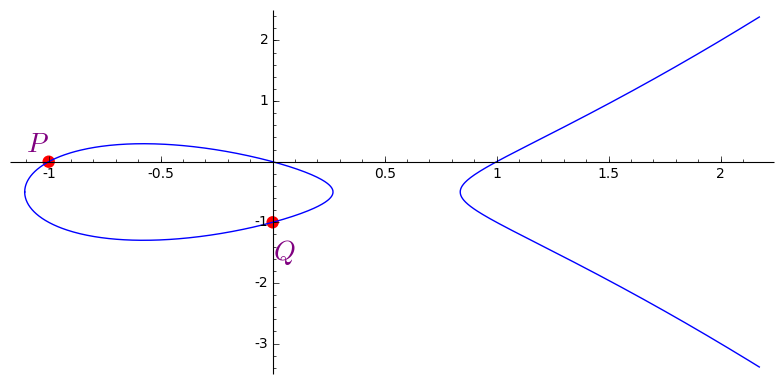
\includegraphics[width=0.8\linewidth]{pics/1.png}
%\end{frame}

%\begin{frame}
%\frametitle{Group law on elliptic curves(II)}
%\centering
%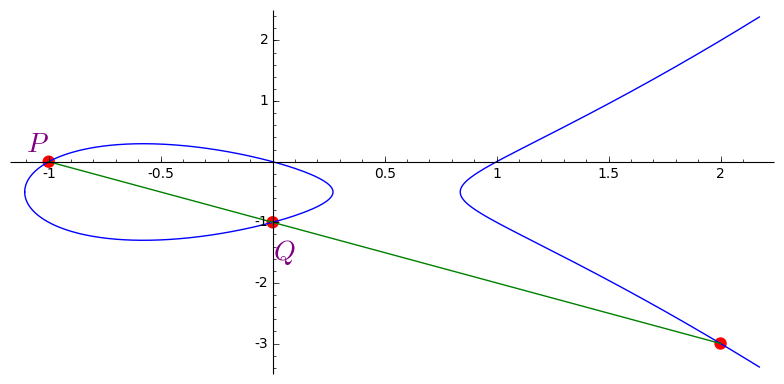
\includegraphics[width=0.8\linewidth]{pics/2.png}
%\end{frame}

\begin{frame}
\frametitle{The BSD conjecture} 


% $rank(E(\bQ))$ has been studied extensively in number theory. \\ % up to now, no easy way of computing the rank.

\medskip

For every elliptic curve $E/\bQ$, there is an analytic function $L(E,s)$ in the complex variable $s$, called the {$L$-function of $E$}. The rank part of the  {\bf Birch and Swinnerton-Dyer (BSD) conjecture} is:
\begin{equation*}
	rank(E(\bQ)) = \ord_{s=1}L(E,s).
\end{equation*}

\pause

LHS is the {\bf algebraic rank}, RHS is the {\bf analytic rank}, denoted by $r_{an}(E)$. \\

\medskip

\pause

The BSD conjecture is still open when $r_{an}(E) > 1$. \\

\medskip

\pause

The proof of BSD for $r_{an}(E) = 1$ uses {\bf Heegner points} on {\bf modular curves}.


\end{frame}


%------------------------------------------------

\begin{frame}
\frametitle{Modular curves}
Let $N \geq 1$ be an integer, consider the group 
\[
	\Gamma_0(N) = \left \{ \abcd{a}{b}{c}{d} \in SL_2(\bZ): N \mid c \right\}.
\]
Let $\cH = \{z \in \bC: im(z) > 0\}$ be the complex upper half plane. \\

\smallskip 
\pause

The group $\Gamma_0(N)$ acts on the extended upper half plane $\cH^{*} = \cH \cup \bQ \cup \{\infty\}$
by $(\abcd{a}{b}{c}{d} , z) \mapsto \frac{az+b}{cz+d}$.

\pause
\begin{Def}
The {\bf Modular Curve} $X_0(N)$ is the quotient space
of $\cH^*$ under the $\Gamma_0(N)$-action.
\end{Def}

\pause

\begin{itemize}
\item $X_0(N)$ is a compact Riemann surface. %The genus $g(X_0(N))$ is unbounded as $N \to \infty$.  \\
%$Y_0(N) = \Gamma_0(N) \backslash \cH$ parametrises isomorphism classes of pairs $(E,C)$, where $E/\bC$ is an elliptic curve and $C \subseteq E$ is a cyclic subgroup of order $N$.
\item If $z \in \cH^*$, we use the symbol $[z]$ to denote the corresponding point on $X_0(N)$.
\end{itemize}

%{\bf Cusps} on $X_0(N)$  are the equivalence classes of $ \bQ \cup \{\infty\}$.  There are finitely many 
%cusps. 
%i.e., they are spheres with some handles attached. 
%The number of handles is called the \textbf{genus}.

% Next slide: the modular curve $X_0(4)$ with genus $0$ and $3$ cusps $[0],[\frac{1}{2}],[\infty]$.

\end{frame}




%:
%\begin{frame}[plain]
%\begin{figure}[p]
%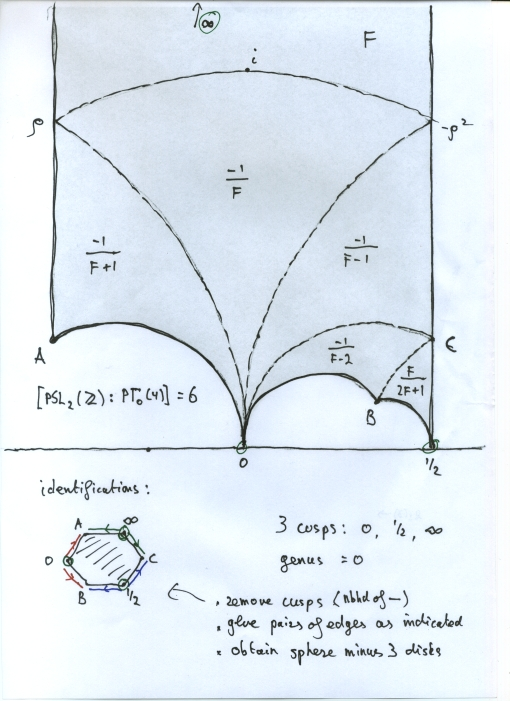
\includegraphics[width=0.8\linewidth]{pics/X0(4).jpg}
%\caption{Picture of the Modular Curve $X_0(4)$}
%\end{figure}
%\end{frame}
%------------------------------------------------

\begin{frame}{Modular functions}

\begin{itemize}
\item $X_0(N)$ is a nonsingular  projective curve defined over $\bQ$.
% So its {\bf function field} $\bQ(X_0(N))$ has transcendence degree 1 over $\bQ$.

\pause
\item Rational functions on $X_0(N)$ are called {\bf modular functions}. Each modular function has a {\bf q-expansion} at $[\infty]$:
\[
	u(q)  = \sum_{n \geq -m} b_n q^n, \; q = e^{2 \pi i z}
\]
which follows from $u(z+1) = u(z)$. 

\pause
\item The {\bf j-invariant} is a modular function on $X_0(N)$ for every $N$, with q-expansion
\[
	j(q) = q^{-1} + 744 + 196884q+ \cdots.
\]
From now on, the letter $j$ means the $j$-invariant. 
% On Y_0(N), we have $j([(E,C)]) = j(E)$.
%The $j$-invariant has poles exactly at the cusps.

\pause

\item If $\omega_1, \omega_2 \neq 0$ are differential forms on $X_0(N)$, then  $\frac{\omega_1}{\omega_2}$ is 
a modular function.  %In particular, $\frac{\omega}{dj}$ is a modular function.
\end{itemize}

\end{frame}

\begin{frame}
\frametitle{The modularity theorem}
%Notation: for a cusp form f weight 2 and level $N$, let $\omega = f(z)dz$.

%\begin{Fact}
%$\omega$ is a holomorphic differential on $X_0(N)$.
%\end{Fact}

\begin{theorem}[Modularity]
For every elliptic curve $E/\bQ$, there exists an integer $N > 1$ and a surjective morphism 
$\varphi: X_0(N) \to E$ defined over $\bQ$.
\end{theorem}
\pause


\begin{itemize}
\item Let $\omega = \omega_{E, \varphi} = \varphi^*(\frac{dx}{y}) $. Then $\omega$ is a holomorphic differential on $X_0(N)$.

\pause

% (For experts: $\omega  = c f(z) dz$, where $f$ is the modular form attached to $E$). 
\item $\omega$ has a q-expansion $\omega = \left( \sum_{n \geq 0} a_n q^n \right) dq$, where the coefficients $a_n$ depend on $E$. Moreover, there exists an algorithm to compute 
this q-expansion.

\pause
\item The smallest $N$ is called the {\bf conductor} of $E$. 

\pause

\item $\varphi$ is called a {\bf modular parametrisation}. \\
We assume $E$ is optimal, then $\varphi$ is unique up to sign.
 %$f(z)$ is {\bf the modular form attached to $E$}   
% We assume $(E,\varphi)$ is a Weil curve, i.e., any non constant map $\psi: X_0(N) \to E'$ to an elliptic curve $E'$ factors through $\varphi$. In this case $\varphi$ is unique upto $\pm 1$. 

\pause 

\item From now on, we fix  the curve $E$, the conductor $N$, the differential $\omega$, and the morphism $\varphi$. 
\end{itemize}


\end{frame}

\begin{frame}{Heegner points}
%Let $D$ be a negative discriminant and let $z \in \cH$ be a solution to $Az^2+Bz+C = 0$, where $A,B,C \in \bZ$, $gcd(A,B,C) =1$,  and $B^2-4AC = D$.  Then it's a fact that $j(z)$ is an algebraic integer. \\

%Let $D$ be a negative integer, such that there exists an imaginary quadratic order
%$\cO_D$ of discriminant $D$. \\
%Let $D < 0$ be an integer of the form $-c^2d$, such that $c,d \in \bZ_{>0}$, $d$ is square free, and $d \equiv 3 \pmod{4}$ if $c$ is odd. 
For an imaginary quadratic order $\cO = \cO_D$ of discriminant $D < 0$, 
let $H_D(x)$ denote its {\bf Hilbert class polynomial}.

\pause
\smallskip


% The {\bf Hilbert class polynomial} of discriminant $D$ is $H_D(x)  = \mbox{ the minimal polynomial of }j(z)$. $H_D(x) \in \bZ[x]$ is monic.
 

\begin{Def}
A point $[z] \in X_0(N)$ is a {\bf ``generalized Heegner point''} if there exists $D$ s.t.
$H_D(j(z)) = H_D(j(Nz)) = 0$. 
If in addition, $(D,2N) = 1$, then $[z]$ is a {\bf Heegner point}.
\end{Def}
\pause 

\end{frame}
% Note: the elliptic points, when they exist, are Heegner points on $X_0(N)$.

% nothing to do with level.
%From the Gross-Zagier formula, we can derive:

\subsection{The critical subgroup and critical polynomials}

\begin{frame}{The critical subgroup $E_{crit}(\bQ)$}
%\frametitle{Background: Ramification}

%Given any morphism $\varphi: X \to Y$ between curves, the ramification divisor of $\varphi$ is 
%\[
%	R_\varphi = \sum_{x \in X} (e_\varphi(x) - 1) [x]
%\]
%there is a finite set of points $x \in X$ where 
%the preimage $\varphi^{-1}(\varphi(x))$ is `smaller than usual'. Such x is called a {\bf critical point}, 
%and $f(x)$ is called a ramification point. 
%For example, the projection $\{(x,y) \in \bR^2: x = y^2\} \to \bR: (x,y) \mapsto x$ 
%is ramified at $(0,0)$.

%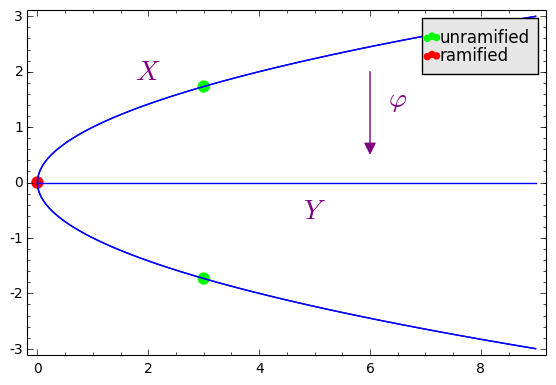
\includegraphics[width=10cm,height=7cm]{pics/ramification.png}


%\end{frame}

%\begin{frame}{Riemann-Hurwitz Formula}
%Some of on divisors: 
%\begin{itemize}
%\item A {\bf divisor} $D$ on a curve $X$ is a finite formal sum of points $D = \sum_{x \in X} n_x[x]$, $n_x \in \bZ$.\\
%\item $\supp D = \{x: n_x \neq 0\}$ = the {\bf support} of the divisor. 
%\item For $f \in \bQ(X)$, $\Div(f) = \{\mbox{zeros of } f\} - \{\mbox{poles of } f\}$.
%\item Divisor of differentials are defined similarly. 
%\end{itemize}

%For every $\varphi: X \to Y$, there exists a divisor $R_{\varphi} \geq 0$, called 
%the \textbf{ramification divisor} of $\varphi$, such that 
%$\supp R_{\varphi} = \mbox{ critical points of } \varphi$.

%\begin{theorem}[Riemann-Hurwitz formula]
%If $\varphi: X \to Y$ is a non-constant morphism of curves and $\omega$ is any differential on $X$, then 
%\[
%          \Div(\varphi^*(\omega))   = \varphi^*(\Div(\omega)) + R_{\varphi}.
%\]
%\end{theorem}
% Let $\varphi: X_0(N) \to E$ be the modular parametrisation and let 


Let $R_\varphi =  \sum (e_\varphi(z)  -1) [z]$ be the ramification divisor of $\varphi$.

\smallskip

Points in $\supp R_{\varphi}$ are called {\bf critical points} in this talk.

\pause

\begin{Def}[Mazur, Swinnerton-Dyer]
The {\bf critical subgroup} of $E$ is
\[
	E_{crit}(\bQ)  = \langle tr(\varphi([z])) : [z] \in \supp R_\varphi \rangle, 
\]
where $tr(P) = \sum_{\sigma: \bQ(P) \to \bar{\bQ}} P^{\sigma}$.
\end{Def}

\pause



\begin{itemize} 
\item $E_{crit}(\bQ)$ is a subgroup of $E(\bQ)$.
%\item $R_\varphi$ is a rational divisor. Therefore, for any $e\in \supp R_\varphi$, we have $\varphi(e) \in E(\bar{\bQ})$.
%\item C.Delaunay described an algorithm to compute $R_\varphi$ using a complex analytic method.
\item $R_\varphi = \Div(\omega)$. In particular, $\deg R_{\varphi} = 2g(X_0(N))-2$. \\
\item From now on, we use the notation $\Div(\omega)$ instead of $R_\varphi$.
\end{itemize}
%Riemann-Hurwitz formula + $\Div(\omega_E) = 0$  $\implies .
%(a canonical divisor on $X_0(N)$). \\

%$\varphi$ is ramified at $2g-2$ points, counting  multiplicity.
%  F.Brunault: a sufficient condition such that $R_\varphi$ 
%does not contain cusps.

\end{frame}

\begin{frame}{Motivation}
Why consider the critical subgroup? 


\pause

\begin{theorem}
(1) If $r_{an}(E) = 1$, then there exists a Heegner point $[z]$ on $X_0(N)$ such that  $tr(\varphi([z])) \in E(\bQ)$ has infinite order.  \\
(2) If $r_{an}(E) \geq 2$, then $tr(\varphi([z])) \in E(\bQ)_{tors}$ for every  ``generalized Heegner point'' $[z]$ on $X_0(N)$.
\end{theorem}

\pause

\begin{itemize}
\item Part (1) is essential to the proof of BSD  for $r_{an}(E) = 1$.
\item When $r_{an}(E) \geq 2$, one can not obtain a non-torsion point using Heegner points. 
\end{itemize}
\pause

What if we use critical points? A natural question is

\begin{question}
Is there an elliptic curve $E/\bQ$ with $r_{an}(E) \geq 2$ and $rank(E_{crit}(\bQ)) >0$?
\end{question}

 % Then he uses a complex form of modular parametrisation to compute $E_{crit}(\bQ)$.

\end{frame}

%------------------------------------------------





\begin{frame}{Critical $j$-polynomial}
%The group $E(\bQ)$ has been studied extensively in number theory.
%Associated to $E$ is an analytic function $L(E,s)$( the L-function of E). \\
%The rank part of the B-SD conjecture states
%\[
%	rank(E(\bQ)) = \ord_{s=1}L(E,s).
%\] 
%It is proved for $\ord_{s=1}L(E,s) \leq 1$.


%\end{frame}

%\subsection{Critical Polynomial}
%\begin{frame}
%\frametitle{Critical Polynomials}

%Notation: $Z_\omega =$.  \\
Plan: investigate $E_{crit}(\bQ)$ by studying the `critical $j$-polynomial' attached to $\Div(\omega)$. 

\pause 
\begin{Def}
%Let $E/\bQ$ be an elliptic curve of conductor $N$ and let $j$ be the $j$-invariant. 
Write $\Div(\omega) = \sum n_z[z]$. The \textbf{critical j-polynomial} of $E$ is 
\[
F_{E,j}(x) = \prod_{z \in \supp \Div(\omega), j(z) \neq \infty}(x-j(z))^{n_z}.
\]
\end{Def}

\pause 
\begin{itemize}
\item $F_{E,j}(x) \in \bQ[x]$.
\item $\deg F_{E,j} \leq 2g-2$. Equality holds if $N$ is square free.
\item If $h \in \bQ(X_0(N))$ is a non-constant function, then
$F_{E,h}(x)$ is defined similarly.						
\end{itemize}

\pause

What next? We will give an algorithm to compute $F_{E,j}$.
%So two natural questions are:
%\begin{question}
%What information can we obtain about $\Div(\omega)$ using computational methods? How do we use these information to the study of $E_{crit}(\bQ)$?
%\end{question}

\end{frame}

%------------------------------------------------

\begin{frame}{Polynomial Relation ({\bf PR}): a proposition}
%When  $N$ is not square free, \textbf{NORM} does not work. \textbf{IPR} is an algorithm to compute $F_{E,j}$, which works for any $N$. \\

Fact: Let $C/\bQ$ be a nonsingular projective curve, $r \in \bQ(C)$ be a non-constant function, then $[\bQ(C): \bQ(r)] = \deg r$.

%The {\bf degree} of $x$, denoted by $\deg(x)$, is the number of zeros(or poles) of $x$(counting multiplicity). 
\pause 

\smallskip


Let $r, u$ be non-constant functions on $C$, a {\bf minimal polynomial relation} of $r$ and $u$ is an irreducible polynomial $P(x,y) \in \bQ[x,y]$, with \hyperlink{proof: minimal pr}{$\underline{\deg_x(P) \leq \deg u, \deg_y(P) \leq \deg r}$}, such that $P(r,u) = 0$.  \\

\pause 
\smallskip
Remark: The minimal polynomial relation always exists and is unique up to multiplication by a constant.

\pause 

\hypertarget{pr: prelim}{}

Write $\Div(r) =  \sum n_z[z]$ and $P(x,y) = f_n(y)x^n + \cdots + f_1(y)x + f_0(y)$. 


\begin{Prop}[C.]
\label{mult}
If $\bQ(C) = \bQ(r,u)$ and $\gcd(f_0(y), f_n(y)) = 1$, then there is a constant $c \neq 0$ s.t.
%$\Div_{\infty}(r) \subseteq \Div_0(u)$,
\[
		f_0(y) = c \prod_{z \in\Div_{0}(r) \setminus \Div_{\infty}(u)} (y - u(z))^{n_z}.
\]
%(2) Let $K$  be a finite Galois extension of $\bQ(u)$ containing $\bQ(r,u)$ and $\{r_1 = r, r_2,  \cdots, r_n \} \subseteq K$ be the conjugates of $r$ over $\bQ(u)$. Suppose $\Div_0(r_i) \cap  \Div_{\infty}(r_j) = \emptyset$ for all $i, j$, then $\gcd(f_0(y), f_n(y)) = 1$ and the conclusion of (1) holds.
\end{Prop}


\end{frame}

\begin{frame}{Polynomial Relation: a proposition (II)}

Recall the proposition just stated.
\begin{Prop}[C.]
\label{mult}
If $\bQ(C) = \bQ(r,u)$ and $\gcd(f_0(y), f_n(y)) = 1$, then there is a constant $c \neq 0$ s.t.
%$\Div_{\infty}(r) \subseteq \Div_0(u)$,
\[
		f_0(y) = c \prod_{z \in\Div_{0}(r) \setminus \Div_{\infty}(u)} (y - u(z))^{n_z}.
\]
%(2) Let $K$  be a finite Galois extension of $\bQ(u)$ containing $\bQ(r,u)$ and $\{r_1 = r, r_2,  \cdots, r_n \} \subseteq K$ be the conjugates of $r$ over $\bQ(u)$. Suppose $\Div_0(r_i) \cap  \Div_{\infty}(r_j) = \emptyset$ for all $i, j$, then $\gcd(f_0(y), f_n(y)) = 1$ and the conclusion of (1) holds.
\end{Prop}


\smallskip
\pause

%\begin{remark}[The conditions are necessary]
%(1) If $r = u$, then $P(x,y) = x- y$, and $f_0(y) = -y$ has degree 1. So if $\deg(r) > 1$, then the claim in the proposition is false. This shows the condition $\bQ(r,u) = \bQ(C)$ is necessary. \\
%(2) Consider $C = (\frac{1}{2}yx^2 - xz^2 - \frac{1}{2}y^2z = 0)$ and 
%$r = \frac{x}{z}, u = \frac{y}{z}$. Then $\Div(r) = (0:0:1) -(1:0:0)$, and $\Div(u) = (0:0:1) -(0:1:0)$. So the right hand side should have degree 1, but $f_0(y) = -\frac{1}{2}y^2$ has 
%degree 2. This shows that the condition $(f_0, f_n) = 1$ is necessary.
%\end{remark}

\begin{itemize} 
\item The right hand side `looks like a critical polynomial'. 


\pause


\item We will apply the proposition to compute $F_{E,j}$. \\

%\item To this purpose, we need to divide $\omega$ by some differential on $X_0(N)$ to obtain a modular function. \\
%\item We can use $dj$.
\end{itemize}
%But it is a product over the zeros of a function, not of a differential... 
% The proof uses extension of valuations.
\end{frame}

%------------------------------------------------



\begin{frame}{Polynomial Relation: theorem}
Let $C = X_0(N)$ and let $dj = j'(z)dz$. Set
\[
r = j(j-1728)  \frac{\omega }{{dj}}, \;  u = \frac{1}{j}.
\]
Then $r, u \in \bQ(X_0(N))$, and $\Div_0(r)  = \Div(\omega) + D_0$, where points in $\supp D_0$ have $j$-value 0 or 1728.  \\

\smallskip 

\pause

%Moreover, if $T >  2g-2$, then the pair $(rj^T,u)$ satisfies the conditions of the proposition. (\hyperlink{condition is satisfied}{\underline{One proves it by looking at the zeros and poles of $rj^T$}}). % Proof is not long, but please believe me. t

\begin{theorem}[C.]
If $T \in \bZ_{>0}$ is sufficiently large and $P(x,y) = f_n(y)x^n + \cdots + f_1(y)x + f_0(y)$ is a minimal polynomial relation between $rj^T$ and $u$, then
\[
		F_{E,j}(x) = f_0 ( 1/x) \cdot x^{A} (x - 1728)^B
\]	
where $A,B$ are integers  \hyperlink{consts AB}{depending on $N, P$ and $T$}.


\end{theorem}

\hypertarget{theorem}{}

\end{frame}




\begin{frame}{Polynomial Relation: algorithm}

Algorithm: {\bf PR} \\
Input: the $q$-expansion of the modular form $f_E$ attached to $E$; Output: $F_{E,j}$.  

\pause

\begin{enumerate}
\item $r = \frac{j(j-1728) f_E dz }{dj}, \;  u = \frac{1}{j}$.

\pause

\item Fix \hyperlink{largeM}{\underline{a large $M$}}, compute the q-expansions of $r$ and $u$ to $q^M$.  \\

\pause 
\item Write  $\sum_{\substack{0 \leq a \leq \deg u \\ 0 \leq b \leq \deg r}} c_{a,b}r(q)^au(q)^b = 0 \pmod {q^M} $ as a linear system on the coefficients $c_{a,b}$.

\pause 

\item When $M$ is sufficiently large, the linear system has nullity 1. Let $(c_{a,b})$ be a nonzero solution. 

\pause

\item Set $P(x,y) = \sum c_{a,b}x^ay^b$ and apply the theorem.
\end{enumerate}

\hypertarget{pr: algorithm}{}


\pause

\begin{Example}
$F_{{\bf 44a},j}(x) = H_{-44}(x)^2$. $F_{{\bf 37a},j}(x) = H_{-148}(x)$. $F_{{\bf 37b},j}(x) = H_{-16}(x)^2$.
\end{Example}

\pause

Remark: When $N$ is large($\sim 1000$), the algorithm {\bf PR} is slow. We have 
\hyperlink{yang pair}{\underline{another faster algorithm}} that computes a critical $h$-polynomial, where $h$ is some $\eta$-quotient chosen within the algorithm.

\end{frame}


%\begin{frame}{More examples of critical $j$-polynomials computed via the {\bf IPR} algorithm}
%\begin{Example}
%$E = \textbf{197a}$, we obtain
%\[
%	F_{E,j}(x)  = (x + 884736)^2 H_{-197 \cdot 4}(x) f_{18}(x),
%\]
%where $f_{18}$ is an irreducible polynomial in $\bQ[x]$ of degree 18.
%\end{Example}

%\begin{Example}
%\label{ex: 389a}
%$E = \textbf{389a}$, the curve of algebraic rank 2 with smallest conductor. 
%\[
%	F_{E,j}(x)  = (x + 884736)^2 f_{60}, 
%\]
%where $f_{60}$ is irreducible of degree 60. 
%This example will be revisited in Section ~\ref{sec:exact points}. 
%\end{Example}

%\pause



% \hyperlink{yang pair}{Yang pair}


%\end{frame}

%------------------------------------------------

%\begin{frame}{Integer Polynomial Relation(IPR): Example}
%\begin{Example}
%$E = \textbf{44a}$,
%\begin{align*}
%F_{E,j}(x) &= (x^{3} - 1122662608x^{2} + 270413882112x - 653249011576832)^2  \\
%            &= H_{-44}(x)^2.
%\end{align*}
%\end{Example}

%\begin{Example}
%$E = \textbf{48a}$, $F_{E,j}(x) = 1$. Explanation: All critical points are cusps. In fact, $Z_{\omega}  = [1/4] + [3/4] + [1/12] +[7/12]$. 
%\end{Example}


%\end{frame}


%------------------------------------------------
%\section{Algorithm: Yang pair}

%\begin{figure}
%\includegraphics[width=0.8\linewidth]{test}
%\end{figure}


%------------------------------------------------

%Remark: once we have $F(r_1, h_2) = 0$, let $F_0(x) = F(0,h_2)$. Then $F_{E,h} =  F(0,h_2)/(*)$, where $(*)$ the extra factor  coming from zeros of $h_1$. $(*)$ is explicitly computable, but we may also `eyeball' it. \\




%------------------------------------------------
\subsection{Application of results to $E_{crit}(\bQ)$}

\begin{frame}{The critical subgroup $E_{crit}(\bQ)$: preliminaries}

Recall the definition $E_{crit}(\bQ)  = \langle tr(\varphi([z])) : [z] \in \supp \Div(\omega) \rangle$. \\

\smallskip

%Reason: if $e,e' \in \Div(\omega)$ and $e' \sim e \pmod{Gal(\bar{\bQ}/\bQ)}$, then  $\varphi(e') \sim \varphi(e)  \pmod{Gal(\bar{\bQ}/\bQ)}$, thus $tr(\varphi(e')) = tr(\varphi(e))$. 

\pause

Let $n_{\omega}$ denote the \mbox{ number of Galois orbits of } $\Div(\omega)$. \\
\begin{Fact}
$rank(E_{crit}(\bQ)) \leq n_{\omega}$. 
\end{Fact}
\smallskip

\pause

Reason: to generate $E_{crit}(\bQ)$, it suffices to take one representative from each Galois orbit of $\supp \Div(\omega)$. \\ 





%First, we make a simple observation. 

%\medskip

%Let $E_4, E_6$ be the Eisenstein series of level 1 and weight 4,6. Let $\Delta$ be the discriminant cusp form of level 1 and weight 12. 

% . \\

% Recall the definition: $E_{crit}(\bQ) = \langle tr(\varphi(e)): e \in \supp \Div(\omega)\rangle$. We observe that 

%Write $Z_\omega = \sum_{i = 1}^n n_i S_i$, where the $n_i \in \bZ_{\geq 1}$ and each $S_i$ is a sum of points in a Galois orbit. Set $P_i = \sum \varphi_*(S_i) \in E(\bQ)$. Let $E_{crit}^u(\bQ)  = \langle \{P_i\}_i \rangle$.
%\begin{Lemma}
%$E_{crit}(\bQ) \otimes \bQ = E_{crit}^u(\bQ) \otimes \bQ$, i.e., $E_{crit}^u(\bQ)$ and  $E_{crit}(\bQ)$ have the same rank as abelian groups.
%\end{Lemma}


%\begin{itemize}
%\item Observation: $g = \frac{f\Delta}{E_4^2E_6} \in \bQ(X_0(N))$.  \\
%\item Therefore, $\varphi_*(\Div(g)) = \Div(\varphi_*(g))$(i.e., it is a principal divisor). \\
%\item However, if $D = \sum n_P[P]$ is a principal divisor on $E$, then $\sum n_P P = 0 \in E(\bQ)$. \\
%\item This gives a linear relation on the images of zeros of these four modular forms. 
%\end{itemize}
%\begin{align*}
%& \implies \varphi_*(\Div(g)) = 0 \in Div^0(E) \\
%& \implies \sum_{z \in \Div(g)} n_z\varphi(z) = 0 \in E(\bQ). 
%\end{align*}

\end{frame}


\begin{frame}{The critical subgroup $E_{crit}(\bQ)$: a lemma}
\begin{Def}
Let $[z] \in X_0(N)$, the {\bf period} of $[z]$ is $m_z := \frac{1}{2}|\{\alpha \in \Gamma_0(N): \alpha(z) = z\}|$. If $m_z > 1$, then $[z]$ is an {\bf elliptic point}.
% $[\frac{i}{j i + 1}]$ where $j^2 + 1 \equiv 0 \pmod{N}$, or $[\frac{\rho}{j \rho + 1}]$ where $j^2 - j + 1 \equiv 0 \pmod{N}$ and $\rho = e^{\frac{2 \pi i}{3}}$. 
\end{Def}

\pause

\begin{itemize}
\item elliptic points have period 2 or 3. 
\item the set of elliptic points is finite and Galois invariant. 
\item elliptic points are Heegner points. 
\end{itemize}

\pause
% The proof uses the fact that $g = \frac{f\Delta}{E_4^2E_6} \in \bQ(X_0(N))$. Feel free to  me after the talk about the proof.

Let $P_{all} = \sum_{z \in \supp \Div(\omega)} n_z \varphi([z])$. The point $P_{all}$ is a linear combination of the defining generators of $E_{crit}(\bQ)$. \\

\smallskip
\pause

Let $E_i(N)$ denote the set of elliptic points on $X_0(N)$ of period $i$, (i = 2,3).\\

\pause
\begin{Lemma}[C.]
$6 P_{all} =  - 3 \sum_{c \in E_2(N)} \varphi(c) - 4 \sum_{d \in E_3(N)} \varphi(d)$. \\
\end{Lemma}

\footnotetext[1]{The set of elliptic points can be empty: for example, it happens when $36 \mid N$. It is not always empty, though, since if $k^2 +1 \equiv 0 \pmod{N}$ then $i/(ki+1)$ is an elliptic point of period 2}.
\end{frame}


\begin{frame}{The critical subgroup $E_{crit}(\bQ)$: theorem}
%Recall the lemma: 
%\begin{Lemma}[C.]
%$6 P_{all} =  - 3 \sum_{c \in Ell_2(N)} \varphi(c) - 4 \sum_{d \in Ell_3(N)} \varphi(d)$. \\
%\end{Lemma}

% If $r_{an}(E) \geq 2$, then the right hand side is torsion by Gross-Zagier, hence

\begin{Prop}[C.]
Assume either $r_{an}(E) \geq 2$ or $X_0(N)$ has no elliptic point. Then $P_{all} \in E(\bQ)_{tors}$,  hence $rank(E_{crit}(\bQ)) \leq n_{\omega} - 1$. 
\end{Prop}
\pause

%If in addition $r_{an}(E)$ is even, then $w_N(\varphi(e)) \equiv - \varphi(e) \pmod {E(\bar{\bQ)}_{tors}}$ for all $e \in X_0(N)$.
\begin{Theorem}[C.]
\label{cor: cm}
%Let $E/\bQ$ be an elliptic curve of conductor $N$. 
Suppose $r_{an}(E) \geq 2$, and assume at least one of the following holds: \\
(1) $F_{E,j} = \prod_{m =1}^k H_{D_m}^{s_i}\cdot F_0$, where 
$\bQ(\sqrt{D_m}) \neq \bQ(\sqrt{D_n})$ for all $m\neq n$, and $F_0$ is irreducible. \\
(2) $F_{E,h}$ is irreducible for some non-constant function $h \in \bQ(X_0(N))$. \\
Then $rank(E_{crit}(\bQ))  = 0$. 
\end{Theorem}

\begin{itemize}
\item We make the assumptions of this theorem based on the outputs of the {\bf PR}
algorithm.
\item \hyperlink{proof of cor}{The proof uses the theorem we introduced on trace of Heegner points}.
\end{itemize}
\hypertarget{corollaries}{}
\end{frame}

\begin{frame}{Motivation (II)}

As of now, the only result in the literature on $E_{crit}(\bQ)$ where $r_{an}(E) \geq 2$ is the work of C.Delaunay in 2002, in his Ph.D. thesis. He computed  the divisor $\Div(\omega)$ numerically for $E = {\bf 389a}$, the first elliptic curve of rank 2 over $\bQ$. 

\pause
\smallskip

We quote from Delaunay's paper: \\

"More astonishing, 2 critical points(for {\bf 389a}) are Heegner points. $\cdots$ It also appears that $E(\bQ)^{crit}$ is a torsion subgroup."

\pause
\smallskip

One of my goals is to {\em prove} this statement for {\bf 389a} and investigate the critical subgroup of other elliptic curves. 


\end{frame}
%------------------------------------------------

\begin{frame}
\frametitle{Critical polynomials for elliptic curves of rank 2 and conductor $<1000$ (I)}
\begin{center}
   \begin{table}[h!]
    \begin{tabular}{ | l | l | l | |p{4.4cm}  |}
    \hline
    $E \footnotemark$ & $g(X_0(N))$    & $h$ & $\mbox{ Factorization of } F_{E,h}(x)$     \\ \hline \hline
    389a & 32  & $j$ & $H_{-19}(x)^2 (x^{60}+ \cdots)$ \\ \hline
    433a & 35  & $j$ &  $x^{68}+\cdots$  \\ \hline
     446d & 55  & $j$ &  $x^{108}+\cdots$ \\ \hline
    563a & 47  & $j$ &  $H_{-43}(x)^2 (x^{90} - \cdots)$   \\ \hline
    571b& 47  & $j$ &  $H_{-67}(x)^2 (x^{90} - \cdots)$ \\ \hline
    643a& 53  & $j$ &  $H_{-19}(x)^2 (x^{102} - \cdots)$ \\ \hline
    664a & 81    &   $\frac{\eta_4\eta_8^2 \eta_{332}^5}{\eta_{166}\eta_{664}^{6}{\eta_2}}$ & $x^{160} - \cdots$ \\ \hline
    655a& 65  & $j$ &  $x^{128} - \cdots$ \\  \hline
    681c& 75  & $j$ &  $x^{148} - \cdots$ \\  \hline
    707a & 67  & $j$ & $x^{132} - \cdots$ 
        \end{tabular}
    \label{table: rank two}	
   \end{table}
\end{center}

 \footnotetext[1]{We use Cremona's labels for elliptic curves, where the number represents  the conductor, and the letter represents the isogeny class.}

\end{frame}
 

\begin{frame}
\frametitle{Critical polynomials for elliptic curves of rank 2 and conductor $<1000$ (II)}   \begin{table}[h!]
    \begin{tabular}{ | l | l | l |p{4.4cm} |}
    \hline
    $E$ & $g(X_0(N))$    & $h$ & $\mbox{ Factorization of } F_{E,h}(x)$     \\ \hline \hline
    709a& 58  & $j$ &  $x^{114} - \cdots$\\ \hline
    718b& 89  & $j$ &  $ H_{-52}(x)^2 (x^{172} - \cdots)$\\ \hline
    794a& 98  & $j$ &  $H_{-4}(x)^2 (x^{192} - \cdots)$\\ \hline
    817a& 71  & $j$ &  $x^{140} - \cdots$\\ \hline
    
    916c & 113   & $j$ &$H_{-12}(x)^8(x^{216}+\cdots)$  \\ \hline
    
   % 916c & 113   & $\frac{\eta_2^7  \eta_{458}^5}{\eta_{229}\eta_{916}^6\eta_4^2 \eta_1^3}$ &\footnotemark $(x^2 - 28x + 3664)^2(x^2 + 116x + 3664)^2(x^{216}+\cdots)$  \\ \hline
    
    944e & 115    & $\frac{\eta_{16}^4 \eta_{4}^2}{\eta_8^6}$ & $x^{224} - \cdots$.\footnotemark \\ \hline 
    997b& 82  & $j$ &  $H_{-27}(x)^2 (x^{160} - \cdots)$\\ \hline
    997c& 82  & $j$ &  $x^{162} - \cdots$\\ \hline
    \end{tabular}
    \label{table: rank two}	
   \end{table}
   	\footnotetext[1]{Here 4 of the critical points are cusps, so $\deg F = 2g- 6$.}

\end{frame}

%------------------------------------------------


%All critical $j$-polynomials in the table are of the form $F_{E,j} = f_{CM}f_0$, so $E_{crit}(\bQ)$ is torsion in these cases. \\
%The critical $h$-polynomial for the curves \textbf{664a} and \textbf{994e} are irreducible, hence $E_{crit}(\bQ)$ is torsion for these two curves. \\ 
%The critical $h$-polynomial for the curve \textbf{916c} is not irreducible, but...\\
%the two quadratic factors in its factorisation correspond to CM points on $X_0(N)$ with j-value 54000. Therefore, $E_{crit}(\bQ)$ is torsion as well.  \\

\begin{frame}{Discussion}

From the data and the theorems, we conclude:
\begin{Corollary}
For all elliptic curves $E$ of rank 2 and conductor $N <1000$, the rank of $E_{crit}(\bQ))$ is 0.
\end{Corollary}
\pause

Therefore, it seems hard to find an elliptic curve with $r_{an}(E) \geq 2$ and $rank(E_{crit}(\bQ)) > 0$. 

\pause
\smallskip

However, all is not lost. Some future work:

\pause 

\begin{itemize}
\item Does $F_{E,j}$ always factor into a product of Hilbert class polynomials 
and one irreducible polynomial? 

\pause 

\item What happens if we do the same for $\Div(\omega_g)$ for other modular forms $g$
of level $N$? % \item Characterize ramification at cusps(work in progress).

\pause

\item Use {\bf PR} to compute Fourier expansions of newforms at every cusp(work in progress).

\pause
\item Use {\bf PR} to compute Chow-Heegner points(work in progress).

\pause

\item Use {\bf PR} to compute Weierstrass points on $X_0(N)$.
\end{itemize}
\end{frame}



%------------------------------------------------


\begin{frame}
\Huge{\centerline{Thank you!}}
\end{frame}


% consts AB
\begin{frame}{Constants A and B in the theorem}
\hypertarget{consts AB}{}

$A = \deg f_n - d_N \cdot T - \frac{1}{3}(d_N + 2\epsilon_3(N))$, $B = -\frac{1}{2}(d_N+\epsilon_2(N))$. \\

$d_N  = [SL_2(\bZ): \Gamma_0(N)]$,  $\epsilon_i(N) =$ number of of elliptic points of period $i$ on $X_0(N)$(i = 2,3).

\medskip

\hyperlink{theorem}{\small{Click me to go back}}
\end{frame}


% Extra slides that I may not need.
%----------------------------------------------------------------------------------------

\begin{frame}{The algorithm {\bf Y}ang {\bf P}air}
\hypertarget{yang pair}{}
\hyperlink{pr: algorithm}{\small{Click me to go back}}

Issue: \textbf{IPR} is inefficient when $N$ large. So we introduce the algorithm Yang pair. 

\pause 

% $N \sim 10^3 \implies$ Need to compute kernel of matrix of coefficient size $10^{1400}$ and size 1000.  \\
\begin{itemize}
%\item inspired by a method Yifan Yang used.
\item It does {\em not} compute $F_{E,j}$. Instead, computes $F_{E,h}$. \\
\item $h \in \bQ(X_0(N))$ is chosen within the algorithm. \\
\item It is fast and space-efficient.
\end{itemize}

\pause

% \textbf{IPR-YP} is faster and more space-efficient. 

\begin{Def}[Y.Yang]
Two functions $s,t \in \bQ(X_0(N))$ form a \textbf{Yang pair} if  $\Div_{\infty}(s) = m[\infty],  \; \Div_{\infty}(t) = n[\infty]$ and $gcd(m,n) = 1$.
\end{Def}

\pause

\begin{itemize}
\item Finding polynomial relation of a Yang pair is fast: use a variant of `recursive pole cancellation'. \\
\item Moreover, any Yang pair $(h,h')$ satisfies the assumptions of our proposition. 
\end{itemize}

\pause

Hence if we can find $h_1, h_2 \in \bQ(X_0(N))$ s.t.  (1) $(rh_1, h_2)$ form a Yang pair; (2) $\Div(h_1)$ is known, 
then we can compute $F_{E,h_2}$.
%\begin{enumerate}
%\item Set $c(q) = s^n - t^m$.  
%\item Use power series of form $s^a t^b$ to cancel the highest non-positive power of $q$ in $c(q)$.
%\item Repeat (2) until we have 0. 
%\end{enumerate}
%\begin{figure}
%\includegraphics[width=0.8\linewidth]{test}
%\end{figure}
%\end{frame}
\end{frame}
%------------------------------------------------

\begin{frame}{Use $\eta$-products to construct Yang pairs}
% Answer: Use $\eta$-products!
$\eta$ products = modular function on $X_0(N)$ of the form $\prod_{d \mid N}\eta(dz)^{r_d}$.

\pause 
\begin{Fact}[Ligozat + SAGE]
%\item Their divisor are supported on cusps. 
%\item They form a finitely generated subgroup of $\bQ(X_0(N))^{\times}$.
%\item (Important): 
For every divisor $D \geq 0$ supported on cusps, there exists an explicitly computable
$\eta$ product $h$ s.t.  $\Div(h) = D + D' - m[\infty], D' \geq 0$. 
\end{Fact}

\pause 
Using this fact , one can find two $\eta$ products $h_1$,$h_2$ s.t. \\
(1) $r_1 = rh_1$ has only pole at $[\infty]$. \\
(2) $\Div_0(h_2) \geq \Div_\infty(j) -[\infty]$. \\
Now either $(rh_1,h_2)$ or $(rh_1, jh_2)$ is a Yang pair.

\pause

\begin{Example}
$E = \textbf{664a}$ with rank = 2, use $h_2 = \frac{\eta_4\eta_8^2 \eta_{332}^5}{\eta_{166}\eta_{664}^{6}{\eta_2}}$.\\
%$\deg(r_1)  = 247, \deg(h_2) = 103$.  \\
%$F(0,x)  = (x - 166) (x - 2) (x + 2) (x + 166) x^{83} F_{E,h_2}(x)$. \\ 
$F_{E,h_2}(x) = x^{160} - 14434914...196444x^{158} - \cdots$  is irreducible. 
\end{Example}

\hyperlink{pr: algorithm}{\small{Click me to go back}}


\end{frame}

% modular forms
%----------------------------------------------------------------------------------------

\section{$q$-expansion of newforms at non-unitary cusps} 

\AtBeginSection[]
{
 \begin{frame}<beamer>
 \frametitle{Plan}
 \tableofcontents[currentsection]
 \end{frame}
}


\subsection{Problem description}

\begin{frame}
\frametitle{Modular forms}
Let $f$ be a function $f: \cH \to \bC$,  $\alpha  = \abcd{a}{b}{c}{d} \in SL_2(\bZ)$, and let $k \in \bZ$. The weight-k action of $\alpha$ on $f$ is
defined by
\[
	f|[\alpha]_k(z) := (cz+d)^{-k}f(\alpha z).
\]

\pause

\begin{Def}
A \textbf{modular form} of weight $k$ and level $N$ is a holomorphic function $f: \cH \to \bC$ s.t. \\
(1) $f(z)  = f|[\alpha]_k(z), \; \forall \alpha \in \Gamma_0(N)$. \\
(2) $f$ has holomorphic extension to all cusps of $X_0(N)$. \\
\end{Def}

\pause

{\bf Cusp forms} = modular forms that are zero at all cusps. \\
Modular forms have {\bf q-expansions}: $f(q) = \sum_{n \geq 0} a_n q^n$, $q = exp(2\pi i z)$.
\end{frame}


\begin{frame}{Hecke}

\end{frame}

\begin{frame}{Newforms}

\end{frame}

\subsection{Fourier expansions}

\begin{frame}{Fourier expansion}

\end{frame}

\begin{frame}{Idea of computing}

\end{frame}


\begin{frame}{Idea (ctnd)}

\end{frame}

\subsection{Computing twists and pseudo-eigenvalues}

\begin{frame}{Algorithm for twists}

\end{frame}

\begin{frame}{Algorithm for pseudo-eigenvalue}

\end{frame}

\subsection{Examples}

\begin{frame}{Examples (I)}

\end{frame}


\begin{frame}{Examples (II)}

\end{frame}

\subsection{Relations to automorphic side}

\subsection{Further questions}


%----------------------------------------------------------------------------------------

\section{Chow-Heegner points}

\subsection{Definitions}

\subsection{Even index of Chow-Heegner points}

\subsection{Computing Chow-Heegner points}

\begin{frame}{Darmon et al. , Stein}
asdf
\end{frame}

\begin{frame}{My algorithm}

\end{frame}

\begin{frame}{An example}

\end{frame}

\begin{frame}{Future work}

\end{frame}


\end{document} 